\graphicspath{ {./images/} }
\chapter{背景}
\label{c:background}

\section{區塊鏈}

在區塊鏈網路中的每一個全節點(full node)都會維護一份完整的賬本,
賬本記錄了過往所有區塊中的交易,由此我們能夠知曉交易發生的時間點、交易的付款人收款人、交易的金額,
付款人得以向付款人證明自己確實已經付款。

區塊鏈中的資料主要由交易構成,一個交易的生命週期如下:

\begin{enumerate}
  \item 生成
  \item 廣播
  \item 礦工驗證並包入區塊
  \item 成為區塊鏈的一部分,供後人查詢歷史
\end{enumerate}

為了能夠完成這些工作,節點必須快速地檢索交易,因此,一個一個區塊的尋找是不切實際的, 
通常節點會內置一個資料庫,資料庫的索引能夠高速完成查詢工作。

以下分別討論執行生成、驗證、查詢這三項工作時,節點必須儲存哪些資料。

\subsection{交易生成}

在 UTXO 系統中,付款人會找到自己能控制的 UTXO ,
附上收款人地址後簽章。節點會根據錢包中的私鑰持續追蹤自己能花用的 UTXO ,
如果錢包新增私鑰,則節點必須從新掃描所有交易來得到可用的 UTXO。

在賬戶(account)系統中,付款人則直接寫入金額與收款人後簽章。
節點僅需要追蹤付款人的賬戶中的餘額大小。

\subsection{交易驗證}

當每個區塊來臨時,除了驗證區塊頭中的元(meta)訊息是否正確以外,
還會一一驗證區塊中的每一筆交易。

在 UTXO 系統中,節點可以維護一個 UTXO 的集合,對於每一筆交易,
節點去驗證交易的輸入是否存在於 UTXO ,並且驗證交易的簽名。

也就是說,驗證交易所需要儲存的狀態是一個集合:

\[state = \{UTXO\}\]

而在支援智能合約的賬戶系統中,對於一般交易,
節點必須知道付款人是否有足夠的餘額;
若涉及智能合約,則需要額外執行合約程式碼,
欲執行合約,節點需要知道當前合約的狀態。

我們可以用一個鍵值對來表示賬戶系統在驗證交易時所需要儲存的資訊:

\[state = f: address\to account \]

給一個地址,我們能得到對應賬戶的資訊,可能是餘額,也可能是智能合約設置的狀態。

\subsection{交易查詢}

最常見的查詢即為

\subsection{以太坊狀態儲存}

TODO: 本小節我們以以太坊為例,說明狀態儲存的細節

\subsection{狀態儲存的問題}

區塊鏈的狀態儲存方式造成了兩個危害

\begin{enumerate}
  \item 佔用硬碟空間大
  \item 驗證交易時需要硬碟隨機存取
\end{enumerate}

\subsubsection{佔用硬碟空間大}

永遠增長的區塊已經對節點維護者造成負擔,比特幣與以太坊佔用的空間都已經超過 200 GB ,
如果在 AWS 上租用機器來運行以太坊節點,每個月需花費 50 - 70 美金,
若這個成本降不下來,慈善節點的數量勢必會不斷下滑,
根據 \url{https://ethernodes.org/} 的資訊,2018 年仍有將近兩萬個節點,2020 年已經下降到七千。

另外一個問題是,以太坊中存在許多智能合約已經不再被使用,例如 EOS 的 首次貨幣發行 (ICO) ,
在發行結束後,該合約已無作用,但所有的全節點卻仍得繼續儲存它的歷史數據。
這類僅有短暫效力的合約這無疑造成了大量的空間浪費。

\subsubsection{需要硬碟隨機存取}
交易中的賬戶地址沒有規則,因此當節點驗證交易,去獲取賬戶狀態時,
必須進行隨機存取,一個區塊中有幾筆交易,就必須進行幾次隨機存取。
傳統硬碟的存取依賴讀寫頭移動跟碟片旋轉,隨機操作的效率低下,
以致於使用傳統硬碟的節點甚至無法跟上以太坊網路 15 TPS (transaction per second) 的交易速度。
不得不使用造價較為昂貴的固態硬碟又進一步加劇了節點維護者的經濟負擔。

\section{無狀態區塊鏈}
為了解決上述問題,區塊鏈社群提出了狀態租賃、狀態修剪、無狀態區塊鏈等等改進方案。

以下介紹無狀態區塊鏈的概念。

無狀態區塊鏈的核心想法在於,節點能否在只儲存區塊頭的情況下,
仍然能夠驗證交易的正確性?

可以的,如果我們在交易中附上一些額外資訊,並且以區塊頭來驗證這些額外資訊無誤,
就能夠利用這些額外資訊來驗證交易的正確性了。

在 UTXO 系統中,可以在每個區塊頭裡都放入當前所有 UTXO 集合所構成的梅克爾樹的根,
而在每個交易中,額外加入了它所用到的所有 UTXO 的梅克爾路徑,
如此,節點就可以藉由計算區塊頭中的梅克爾根以及交易中的梅克爾路徑是否吻合,來推論交易是否有效。

在賬戶系統中,則可以讓所有賬戶狀態構成一顆 Patricia 梅克爾樹或是稀疏梅克爾樹,
並且在區塊頭裡放入根,
在交易中附上付款人的餘額,以及付款人狀態的梅克爾路徑,
如此,就可以確認付款人的餘額,再去看它是否足夠支應本次交易。

\begin{figure}
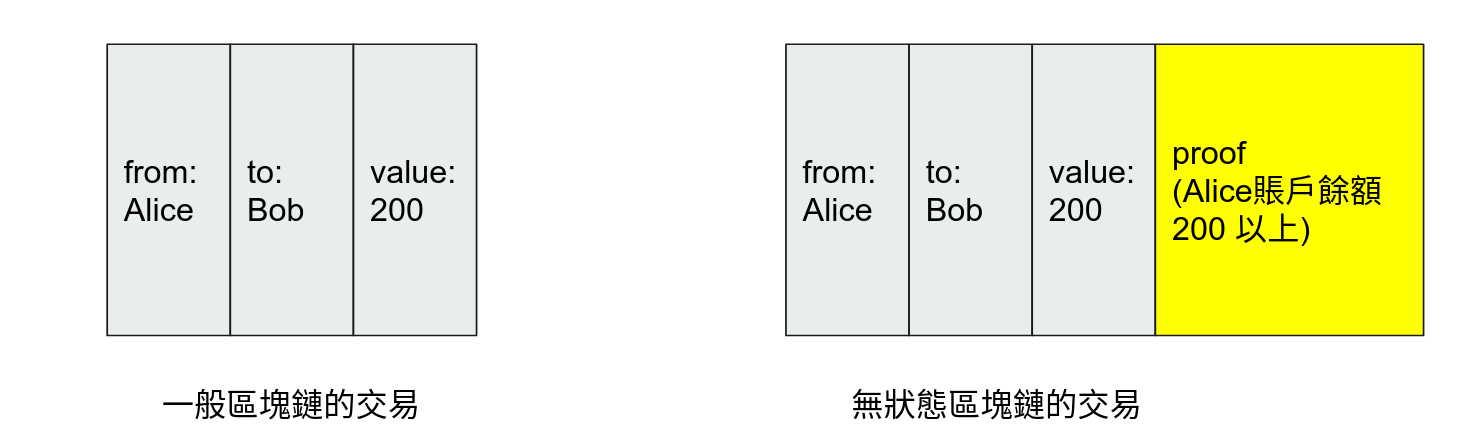
\includegraphics[width=\textwidth]{stateless-tx}
\caption{一般區塊鏈、無狀態區塊鏈交易比較}
\end{figure}

\subsection{accumulator}

accumulator\cite{benaloh1993one} 可以看做是一個集合的摘要

\subsection{vector commitment}

vector commitment\cite{catalano2013vector} 比 accumulator 更強,

近年來 vector commitment 領域也持續出現不同針對無狀態區塊鏈的新構造,
有的能夠將多個證明打包以降低空間\cite{boneh2019batching},
有的則有同態加法的特性,使得製作交易時付款人不用知道收款人的當前餘額\cite{chepurnoy2018edrax}。